\chapter{Testování}

Každý správný vývojový cyklus software obsahuje fázi testování\cite{zivotnicyklus}. Aplikaci lze testovat ve více vlnách, kdy se pokaždé provádí jiný typ testů. Obecně lze testy rozdělit do těchto dvou hlavních skupin - whitebox a blackbox.

Blackbox testy testují aplikaci zvenku a nepotřebují vědět, co se děje uvnitř. Proto se testy označují jako \uv{blackbox}. U těchto testů je aplikace černou skříňkou a jsou k dispozici pouze dva otvory - vstup a výstup. Do aplikace se pošle nějaký vstup a očekává se určitý výstup. Pokud výstup splňuje očekávání, test byl úspěšný. Hlavní výhodou těchto testů je jejich jednoduchost, protože není potřeba znát konkrétní obsah tříd a metod uvnitř aplikace. Do blackbox testů lze zařadit tyto testy:

\begin{itemize}
\item testy rozhraní (Selenium)
\item akceptační
\item zátěžové
\end{itemize}

Naproti tomu whitebox testy vyžadují znalost kódu aplikace a jsou pevněji svázány s implementací uvnitř. Tyto testy jsou mnohem konkrétnější a obvykle testují menší celky aplikace (balíčky -$>$ třídy -$>$ metody). Postup testování může být dvojí. Buď se testují nejdřív největší celky a postupně se zanořuje, nebo se naopak postupuje od nejmenších jednotek po ty největší. Těmto testům se říká jednotkové (angl. unit testy). Do kategorie whitebox testů spadají také integrační testy, které ověřují, zda spolu jednotlivé komponenty aplikace komunikují tak, jak mají.

\section{Použitý způsob testování}

Testování této aplikace není tak snadné jako u webových aplikací. Některé testy nejsou realizovatelné (např. testy rozhraní pomocí nástroje Selenium), protože aplikace není spustitelná v prohlížeči. Toto omezení způsobuje globální objekt Titanium, který není v prostředí prohlížeče k dispozici a aplikace se tak stává nepoužitelnou.

Pro testování je využita JavaScriptová knihovna jsUnity\cite{jsunity}, pomocí které jdou poměrně snadno vytvářet jednotkové testy. Poskytuje jednak běhové prostředí a hlavně assertovací metody, které ověří výsledek testu. Knihovnu je potřeba trochu poupravit, aby výsledek testů vypsala do okna a do výstupu, kde by se výsledek ztratil v záplavě runtime hlášení.

Testy jsou seskupeny v objektech, které se spouští metodou \emph{jsUnity.run()}. Aby nebyly při každém testu znovu zakládány všechny objekty, vytvoří se předem a během testů už se na nich pouze volají metody. Korektní postup je sice jejich zakládání před každým testem v metodě \emph{setUp()}, ale tento způsob se ukázal jako hodně pomalý a bylo od něj upuštěno. Nejpomalejší operace je určitě založení spojení s databází, která je potřeba u většiny testů a protože testy mají být hlavně rychlé, bylo nutné zvolit nějaký kompromis.

\section{Testování asynchronních volání}

V aplikaci se mnoho operací děje asynchronně, aby aplikace nezamrzala (hlavně při spojení se vzdálenými servery). Tento způsob běhu aplikace bohužel znemožňuje testování jednotkovými testy. Asynchronní volání by se dalo rozepsat do těchto kroků:

\begin{enumerate}
\item handler údalosti zavolá metodu na controlleru
\item controller získá potřebná data z databáze a naparsuje je pro potřeby daného serveru
\item pak zavolá metodu \emph{send()} nebo \emph{sendFile()} (pokud se odesílá soubor) na vytvořeném HTTP klientovi. Zároveň mu předá název funkce, kam chce dostat výsledek volání, tzv. callback
\item klient zavolá server s danými parametry a čeká na odpověď
\item po tom, co získá odpověď od serveru, ji naparsuje a pošle zpět controlleru na callback, který od něj získal
\item controller zpracuje odpověď od klienta
\end{enumerate}

Problém, který zabraňuje testování, vzniká v kroku č.3 - předání callbacku. Během testování se o volání metod stará běhové prostředí a není možné volat jednotlivé metody (testy) samostatně. Důsledkem tohoto chování je nemožnost \uv{vrátit} se z HTTP klienta zpět do testu a vyhodnotit správnost odpovědi.

\section{Zátěžové testy}

Součástí fáze testování této práce jsou také zátěžové testy, jejichž úkolem je ověřit, jak rychle některé operace probíhají. Jako operace byla zvolena ta, která je využívána nejčastěji, a sice výpis úkolů z daného projektu. Při používání aplikace se totiž ukázalo, že tato akce trvá poměrně dlouho a zátěžové testy by mohly ukázat, jak moc závažný problém to je.

Zátěžové testy jsou postaveny na podobném principu jako jednotkové testy až na to, že zde se nesleduje výsledek testu, ale pouze jeho průběh. Test probíhá ve více iteracích, aby byla zátěž vystupňována. Bylo vytvořeno celkem 7 scénářů, které byly postupně otestovány:

\begin{itemize}
\item prázdný úkol (bez štítků a přiřazení)
\item úkol s jedním štítkem
\item úkol se dvěma štítky
\item úkol přiřazený uživateli s jedním štítkem
\item úkol přiřazený uživateli se dvěma štítky
\item úkol přiřazený uživateli s pěti štítky
\item úkol přiřazený uživateli s deseti štítky
\end{itemize}

Součástí každé iterace je vložení dalšího úkolu (příp. se štítky a uživatelem) do databáze a zavolání metody, starající se o načítání úkolů z databáze. Tím postupně narůstá zátěž, protože počet úkolů v databázi roste. Iterací bylo při každém testu celkem padesát. Čas spotřebovaný v rámci jedné iterace je měřen pomocí objektu Date a jeho metody getTime(). Tento čas je posléze vypsán na výstup a je dále ručně zpracováván. Hrubá data z těchto testů jsou k nalezení v přílohách této práce. Z těchto hrubých dat byl také pro lepší názornost vytvořen graf, který je vložen níže. Jeho průběh není úplně hladký, což způsobuje pravděpodobně fakt, že testovací prostředí není úplně izolované od dalších procesů běžících na stejném počítači a procesor tak může dát prioritu jiné aplikaci a test se zpomalí. Dalším důvodem může být to, že je nutné číst data z pevného disku (databáze), což může ve stejnou chvíli chtít víc aplikací.

\begin{figure}[h]
	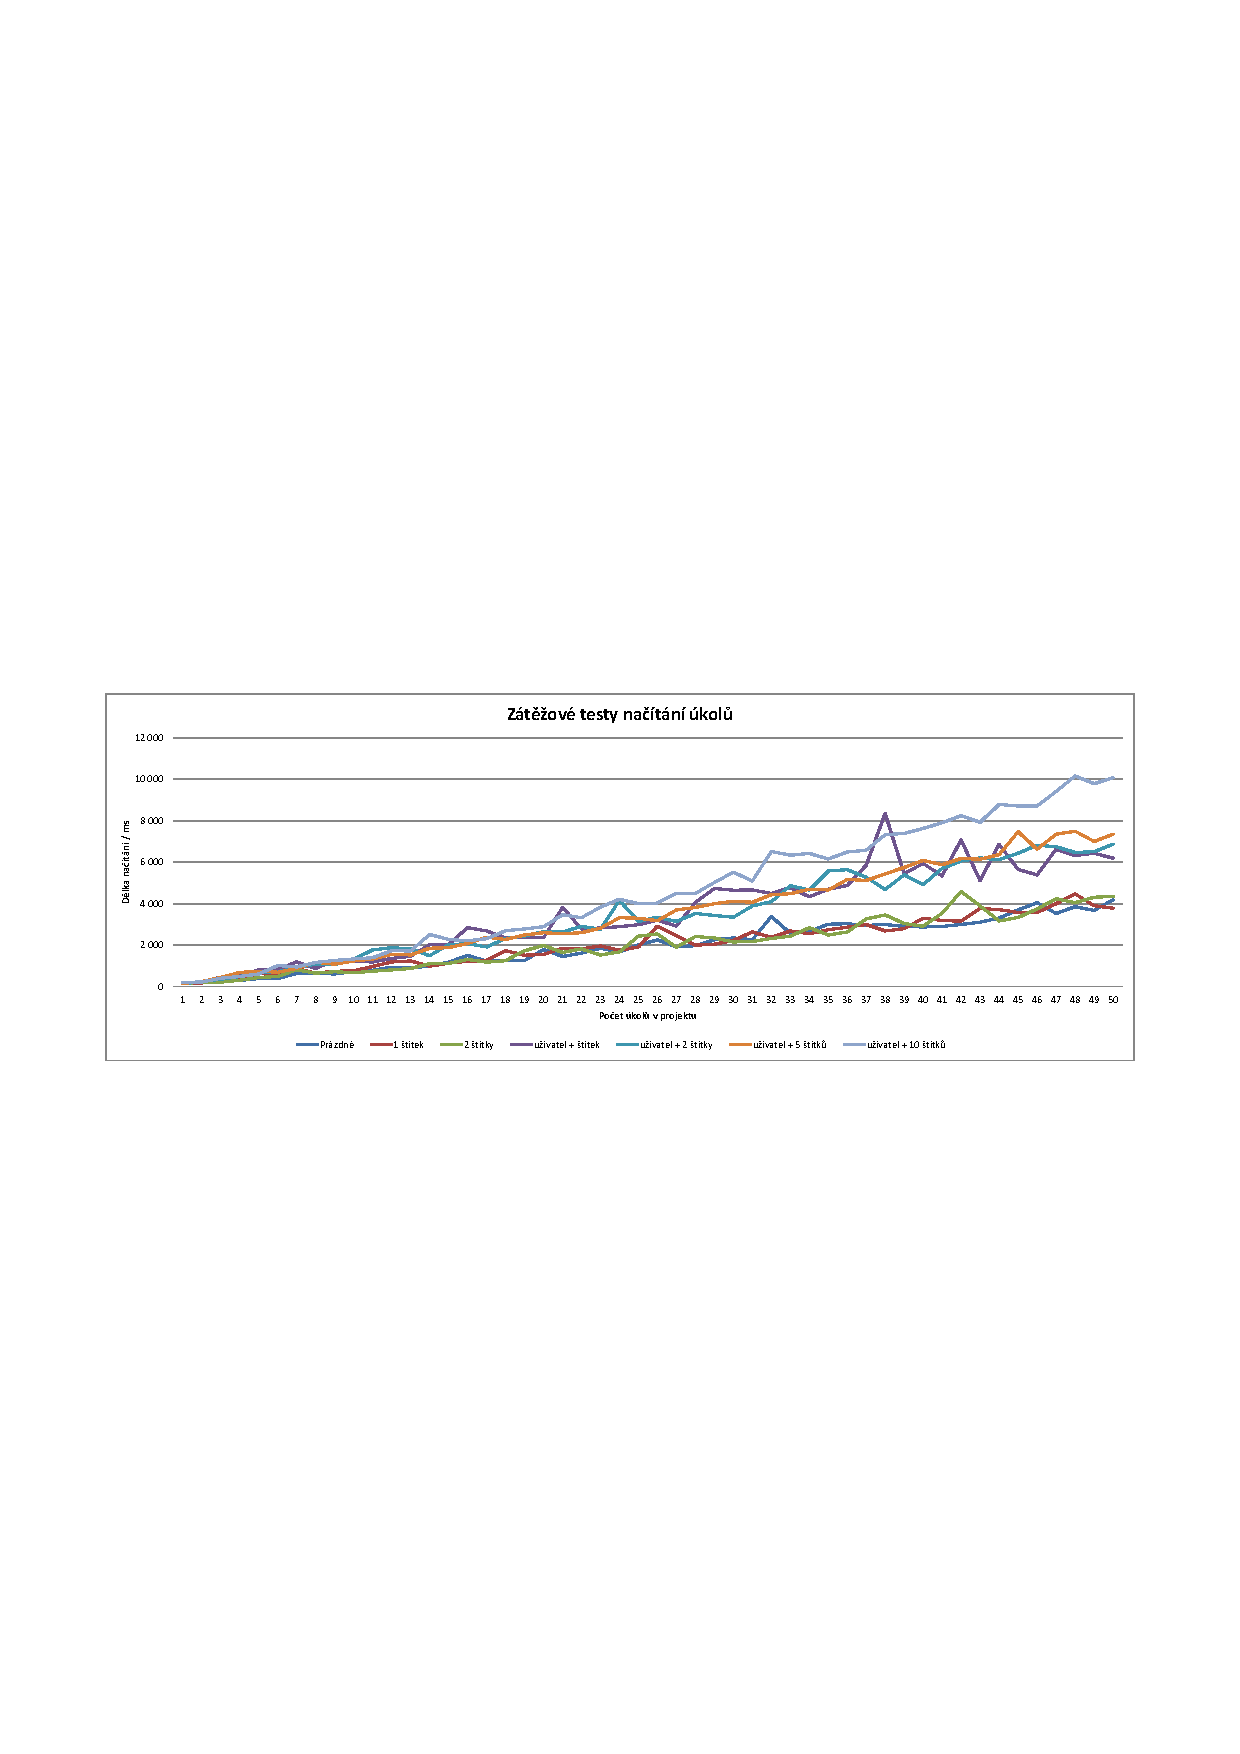
\includegraphics[trim=0cm 11cm 0cm 11cm, clip, width=17cm]{figures/zatezove-testy}
	\caption{Zátěžové testy}
	\label{fig:load-tests}
\end{figure}

\section{Doporučení do dalšího vývoje}

Zátěžové testy ukázaly, že aplikace se stává poměrně pomalou s přibývajícími úkoly v jednotlivých projektech. Problém tkví ve čtení dat z databáze. Řešením by mohla být nějaká vyrovnávací paměť (cache), která by byla umístěna mezi databází a zbytkem aplikace. To s sebou nutně přinese mnoho dalších komplikací a zrychlení aplikace tak může být poměrně drahé. Mezi největší problémy patří určitě volba úložiště vyrovnávací paměti a také její invalidace (smazání neaktuálních dat). Úložiště musí být dostatečně rychle přístupné, aby vůbec mělo smysl vyrovnávací paměť implementovat. Nasnadě je využití souborové cache, ale čtení dat z filesystému nemusí být zrovna nejrychlejší. Lepší by bylo ukládání dat do operační paměti, jenže k té nemá JavaScript přístup. Dalším problémem je invalidace cache, tedy odstranění neaktuálních dat z paměti. Je totiž poměrně velký problém určit, kdy už data nejsou aktuální.

Další funkce, na které se přišlo během vývoje a které byly zařazeny do kategorie \uv{hezké mít} (angl. nice-to-have) jsou tyto:

\begin{itemize}
\item sledování i cizích projektů
\item vytváření vlastních přehledů úkolů (kombinace štítků a projektů)
\item automatické sledování commitů do synchronizovaného repozitáře
\item modulárnější vizuální stránka s využitím knihovny MustacheJS\cite{mustache}
\end{itemize}

Tyto funkce se ukázaly buď jako obtížně realizovatelné (vyrovnávací paměť, vytváření vlastních přehledů) nebo poměrně zbytečné (MustacheJS, sledování commitů), ale přesto byly uloženy, aby se na ně nezapomnělo.